% !TeX root = ../main.tex
% !TeX encoding = UTF-8
% !TeX spellcheck = en_US
% !TeX program = pdflatex

\section{Flat Segmentation Metrics}
For evaluating the performance of flat segmentations, the community has adopted the boundary hit rate for evaluating boundary retrieval, and the pairwise clustering score and V-measure for evaluating the labeling of segments.
The boundary hit rate metric already uses a frameless formulation, and therefore we focus our attention on the two metrics that focus on labeling.
This above connecting text needs some work...
The goal here is to move into definition of PFC and V-measure.

\subsection{Clustering Metrics}
Introduced to the task of music segmentation by Levy and Sandler~\cite{levy2008structural}, the pairwise clustering metric is a standard metric for evaluating a clustering against a reference clustering for elements in a set.

The task of producing a labeled segmentation can be seen as a partitioning a set into labeled clusters, where the set being partitioned is the time span the segmentation occupies.
The original conception of pairwise clustering was formulated with sets of discrete elements, which in the original current version adapted by the community is represented as labels sampled over time, with a frame size of 0.1 seconds.
However, we can formulate this metric with sets consisted of continuous time spans.

\subsection{Notation}
We modify the notational framework set out by prior literature~\cite{DBLP:journals/tismir/NietoMWSSGM20,DBLP:journals/tismir/KinnairdM21} slightly to adapt to a continous time formulation of sets.

For a piece of music with time span \(T = [t_0, t_1]\), a segmentation $S$ has a label mapping $L(t)$ that maps time points in $T$ to the set of unique labels $\gamma = \{y_1, y_2, \ldots\}$ that are used by the segmentation.
\begin{equation}
    L(t): T \to \gamma \label{eq:L}
\end{equation}


% Notice that $L(t)$ is a piecewise constant function, and changes in $L(t)$ define boundaries in $S$.
% The set of boundaries $\beta$ is a superset of the set of change points in $L$.
% \begin{align*}
%     \beta &:= \{b \in T\} \cup \{t_0, t_1\}, \quad \mbox{where}\\
%     \beta &\supseteq \{b \in T | L(t) \neq L(t + \epsilon), \forall \epsilon > 0\}
% \end{align*}



\subsection{Pairwise Clustering}
The pairwise clustering metric (PFC) is a measure of the agreement between two segmentations $S$ and $\hat{S}$.

We denote the set of time pairs $(u, v)$ that are labeled identically by $S$: 
$$\mathcal{A}(S)= \{(u, v)|L_S(u)=L_S(v)\}$$
Pairwise frame clustering metrics are then defined as follows: 
\begin{align*}
\text{PFC}_R = \frac{|\mathcal{A}(S) \cap \mathcal{A}(\hat{S})|}{|\mathcal{A}(S)|}&, \quad
\text{PFC}_P = \frac{|\mathcal{A}(S) \cap \mathcal{A}(\hat{S})|}{|\mathcal{A}(\hat{S})|} \\
\text{PFC}_F = &\frac{2}{\frac1{\text{PFC}_R} + \frac1{\text{PFC}_P}}
\end{align*}

Notice $|\mathcal{A}|$ represents the non zero regions in $A(u, v)$, and $|\mathcal{A}(S) \cap \mathcal{A}(\hat{S})|$ represents the pairs in the overlapping areas between the sets.

We plot a segmentation and its $\mathcal{A}(S)$.

\begin{figure}
    \centering
    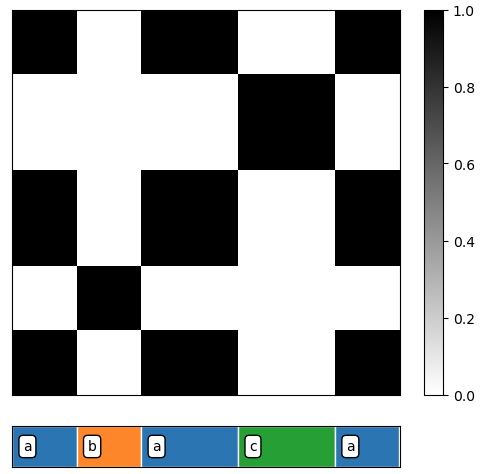
\includegraphics[width=\columnwidth]{content/figs/flat_anno_meet.png}
    \caption{Annotation Agreement Map for the simple Rondo structure represented at the bottom}
    \label{fig:flat_anno_meet}
\end{figure}

\subsection{V-measure}
Inherent from its definition, the PFC metric favors coarser segmentations where its $A(\hat{H})(u, v) = 1$ for large ranges of $u$ and $v$.
This incentivized the adoption of V-measure, another clustering metric, which is the current standard for comparing flat segmentations' labels~\cite{lukashevich2008towards}.
Instead of simply counting occurrences, V-measure looks at the normalized entropy of the true labels conditioned on their estimated label, and vice versa.
For a labeled segmentation $L(t)$ using a set of $k$ labels $\gamma = \{y_1, \ldots, y_k\}$, the entropy of the label distribution can be examined by sampling randomly along its duration:
$$\mathbb{H}(L(t)) = \underset{{y\in\gamma}}{\mathbb{E}}[-\log\mathbb{P}(L(t) = y)]$$
$\mathbb{H}(L(t))$ measures the uncertainty in the distribution defined by $\mathbb{P}(L(t))$ and equals to 0 when the distribution is deterministic (i.e. $L(t) = y_1$ for all $t$). 

$$\mathbb{H}(L_\text{ref} | L_\text{est}) = \underset{y\in\gamma}{\mathbb{E}}[\mathbb{H}(L_\text{ref} | L_\text{est}(t) = y)]$$
is the conditional entropy, which looks at the entropy of reference frame labels only when they receive the same label in the estimate segmentation.
Conceptually, the conditional entropy estimates the amount of uncertainty left in predicting the reference labels given the estimate segmentation.
When the uncertainty for reference label is low given the estimated label, the estimate recalls the labeling information presented in the reference.

V-measure normalizes the conditional entropy by the marginal entropy of the segment labels to calibrate scores for segmentations that have different number of distinct labels.
\begin{align*}
\text{V}_R = 1 - \frac{\mathbb{H}(L_\text{ref} | L_\text{est})}{\mathbb{H}(L_\text{ref})}&, \quad
\text{V}_P = 1 - \frac{\mathbb{H}(L_\text{est} | L_\text{ref})}{\mathbb{H}(L_\text{est})} \\
\text{V}_F = &\frac{2}{\frac1{\text{V}_R} + \frac1{\text{V}_P}}
\end{align*}
